%%%%%%%%%%%%%%%%%%%%%%%%%%%%%%%%%%%%%%%%%%%%%%%%%%%%%%%%%%                                                                                                       	%%
%%   Vorspann						                                               
%%%%%%%%%%%%%%%%%%%%%%%%%%%%%%%%%%%%%%%%%%%%%%%%%%%%%%%%%%

\author{Sergio Vilches}

\title{Compact OCT scanner for a bimodal endoscopic probe}
\hypersetup{pdfkeywords={Endoscopic probe, bimodal, optical coherence tomography, fiber scanner}}

%% Insert Title pic.
\titlepic{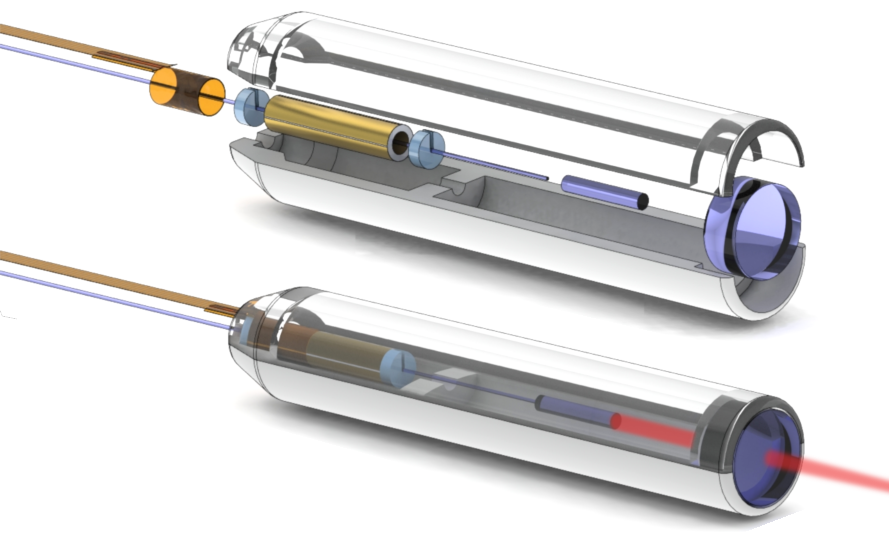
\includegraphics{figures/10_Introduction/explodedRenderTitle.pdf}}
\titlepicdesc{\textbf{Top:} Exploded view of the single modality OCT demonstrator probe.
				\textbf{Bottom:} Render of the assembled probe, showing the optical beampath.}

%%%%%%%%%%%%%%%%%%%%%%%%%%%%%%%%%%%%%%%%%%%%%%%%%%%%%%%%%%%%%%%%%%%%%%%%%%%%%%%%%
%                                                                 Präambel                    																				
%%%%%%%%%%%%%%%%%%%%%%%%%%%%%%%%%%%%%%%%%%%%%%%%%%%%%%%%%%%%%%%%%%%%%%%%%%%%%%%%%

%% Die auskommentierten Varianten sind bei englischer Praeambel zu verwenden
%\dpoversion{20.\,7.~2001}
\dpoversion{July 20, 2009}

%\chair{Lehrstuhl für Mikrooptik}
\chair{Gisela and Erwin Sick Chair of Micro-optics.}

%\referees{Prof.\ Dr.\ Hans Zappe, Lehrstuhl für Mikrooptik\\
%               Prof.\ Dr.\ Zweitkorrektor, Lehrstuhl für Non-sense-research} 
\referees{Prof.\ Dr.\ Hans Zappe, Gisela and Erwin Sick Chair of Micro-optics\\
			Prof.\ Dr.\ Alexander Rohrbach, Bio- and Nano-Photonics research group}

\supervisor{M.Sc.\ Simon Kretschmer, Gisela and Erwin Sick Chair of Micro-optics}

%\thesistime{17.\ Juni 2010 bis 07.\ Januar 2011}
\thesistime{April~1, 2016 to February~23, 2017}


%% Ende Vorspann
